\documentclass[12pt]{article}

\usepackage[a4paper]{geometry}
\usepackage[absolute,overlay]{textpos}
\usepackage{graphicx}
\usepackage{tabularx}
\usepackage{hyperref}
\usepackage{adjustbox}
\usepackage{titling}
\usepackage{float}

\usepackage[version=4]{mhchem}

\newcommand{\subtitle}[1]{%
	\posttitle{%
		\par\end{center}
	\begin{center}\large#1\end{center}
	\vskip0.5em}%
}

\usepackage{fontspec}
\usepackage{unicode-math}

\usepackage{polyglossia}
\setdefaultlanguage{czech}

\def\uv#1{„#1“}

\title{C5966 Vybrané analytické metody a techniky konzervace - cvičení}

\subtitle{Infračervená spektroskopie a termická analýza\\ \url{https://is.muni.cz/www/moravec/c5966/}}

\author % (optional, for multiple authors)
{Zdeněk Moravec, hugo@chemi.muni.cz}

\date{}

\begin{document}
\maketitle

\pagebreak

\section{Průběh cvičení}

	\textbf{Návod není nutné tisknout!}

	Cvičení probíhá v laboratoři C12/112. Doba cvičení je 2--3 hodiny.

	\begin{enumerate}
	\item Krátký úvod k IR spektroskopii \textit{(A12/112)}
	\item Spuštění spektrometrů
	\item Změření IR spektra atmosféry, stanovení vlhkosti uvnitř přístroje
	\item Měření IR spekter vzorků v KBr tabletách a metodou ATR
	\item Interpretace IR spekter
	\end{enumerate}

\subsection{Protokol}

Protokol zašlete na adresu hugo@chemi.muni.cz \textit{do dvou týdnů} ode dne konání cvičení. Optimálním formátem je PDF.

\subsubsection{Doporučená struktura protokolu}

	\begin{enumerate}
	\item Hlavička (Jméno, datum konání cvičení)
	\item Princip
	\item Postup
	\item Spektra (naměřená spektra studenti dostanou v textovém formátu)
	\item Interpretace spekter
	\item Závěr
	\end{enumerate}

\newpage
\section{Infračervená spektroskopie}

Cvičení bude prováděno na přístroji \textit{Bruker Tensor 27}.

\begin{figure}[H]
	\centering
	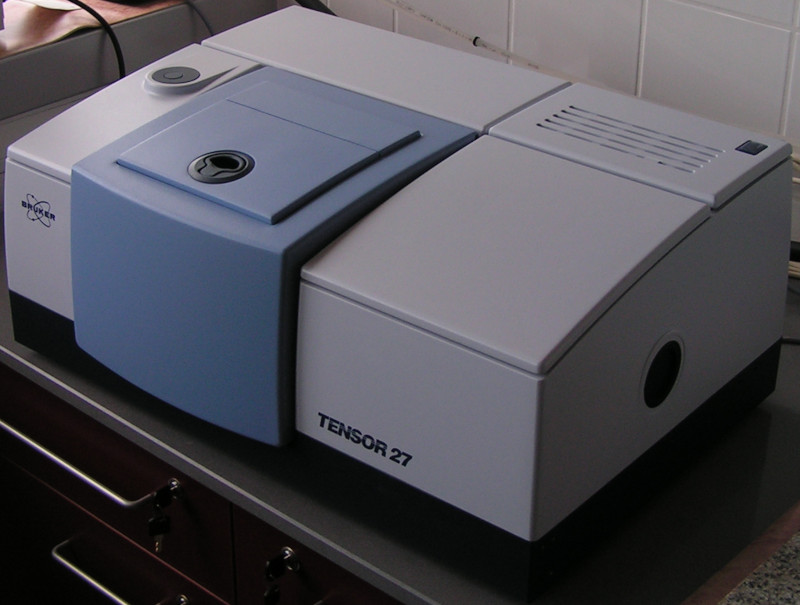
\includegraphics[keepaspectratio,height=8cm]{img/tensor.jpg}
\end{figure}

\subsection{Měření IR spekter vzorků v suspenzi v KBr tabletách}
	1--3~mg vzorku smícháme s cca 300~mg KBr a směs rozetřeme v~achátové třecí misce. Získaný prášek nasypeme do lisovací matrice a lisujeme pod tlakem 8--9 tun po dobu cca 1~minuty.

\begin{figure}[H]
	\centering
	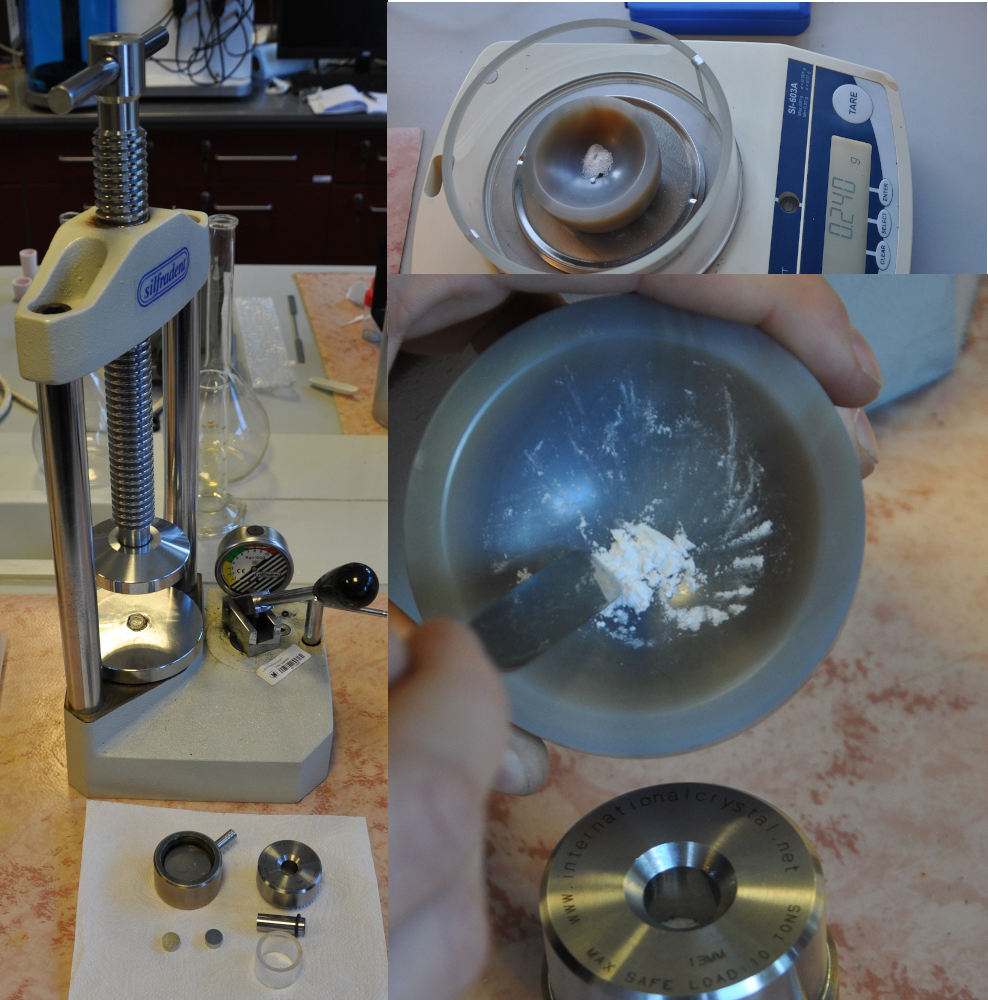
\includegraphics[keepaspectratio,height=10cm]{img/KBr.png}
\end{figure}

\subsection{Měření IR spekter vzorků metodou ATR}
Vzorek nasypeme na krystal diamantu, přitlačíme hrotem a změříme spektrum. Vzorky není potřeba žádným způsobem upravovat.

\subsection{Vyhodnocení}

Studenti dostanou naměřená IR spektra v textovém formátu, úkolem bude vytvořit grafický záznam spektra (doporučuji využít Gnuplot) a přiřadit nejintenzivnější pásy vibracím vazeb v molekule vzorku.

\begin{figure}[H]
	\centering
	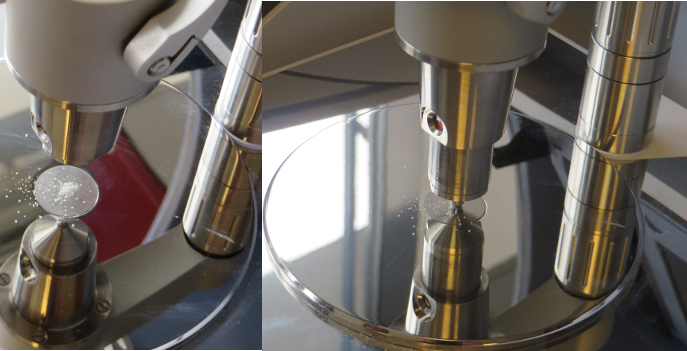
\includegraphics[keepaspectratio,width=9cm]{img/atr.png}
\end{figure}

\newpage
\section{Termická analýza}

Cvičení bude prováděno na přístroji \textit{Netzsch STA 449C Jupiter}.

\begin{figure}[H]
	\centering
	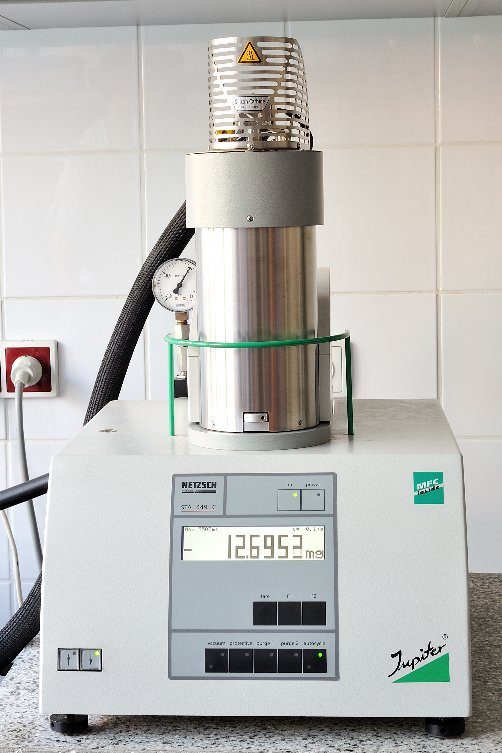
\includegraphics[keepaspectratio,width=47mm]{img/Netzsch.png}
\end{figure}

\subsection{Měření TG/DSC modré skalice}

\begin{enumerate}
	\item Do Pt/Rh kelímku navažte přibližně 5 mg modré skalice. S kelímkem je nutné pracovat opatrně, aby nedošlo k jeho deformaci.
	\item Kelímek s navážkou velmi opatrně umístěte do DSC držáku. Kelímek musí dosednout až na dno.
	\item Pomocí tlačítka Safety a tlačítka s šipkou směrem dolů spusťte pec do měřící polohu.
	\item V měřícím SW nastavte teplotní program podle následujících parametrů:
	\begin{itemize}
		\item Maximální teplota: 1000 $^\circ$C
		\item Teplotní gradient: 10 K.min$^{-1}$
		\item Průtok plynu pecí: syntetický vzduch, 100 ml.min$^{-1}$
	\end{itemize}
	\item Po ustálení vah spusťte měření.
\end{enumerate}

\subsection{Vyhodnocení}
Z naměřeného termogramu odvoďte mechanismus termické degradace modré skalice.

\end{document}